\section{Дополнения}

\subsection{Тензор кривизны Римана}

Мы определяли символы Кристоффеля и ковариантную производную для двумерных поверхностей, а затем получили их выражения через метрику. Можно взять выведенные формулы за определения этих понятий в криволинейных координатах (никак не связанных с поверхностями), переходя таким образом к несколько более общей ситуации. Отметим также, что при выводе этих формул размерность нигде не использовалась, так что далее будем работать с криволинейными координатами в области евклидова пространства $\R^n$.

Зададимся естественным вопросом: можно ли по римановой метрике в области восстановить систему криволинейных координат, метрика которой совпадает с указанной? Ответ следует искать в деривационных уравнениях Гаусса:
\[
	\frac{\partial^2\vec{r}}{\partial u^i\partial u^j} = \Gamma_{ij}^k\frac{\partial\vec{r}}{\partial u^k}.
\]
Действительно, ведь если какая-то матрица претендует быть метрикой криволинейной системы координат, то она должна удовлетворять системе деривационных уравнений, куда она входит через символы Кристоффеля. Запишем для данной системы условия совместности из теоремы Дарбу \ref{theorem:Darboux}:
\[
	\frac{\partial^3\vec{r}}{\partial u^i\partial u^j\partial u^l} = \frac{\partial^3\vec{r}}{\partial u^i\partial u^l\partial u^j}.
\]
Распишем левую часть:
\begin{multline*}
	\frac{\partial^3\vec{r}}{\partial u^i\partial u^j\partial u^l} = \frac{\partial}{\partial u^l}\br{\frac{\partial^2\vec{r}}{\partial u^i\partial u^j}} = \frac{\partial}{\partial u^l}\br{\Gamma_{ij}^k\frac{\partial\vec{r}}{\partial u^k}} =\\ = \frac{\partial\Gamma_{ij}^k}{\partial u^l}\frac{\partial\vec{r}}{\partial u^k} + \Gamma_{ij}^k\frac{\partial^2\vec{r}}{\partial u^k\partial u^l} = \frac{\partial\Gamma_{ij}^k}{\partial u^l}\frac{\partial\vec{r}}{\partial u^k} + \Gamma_{ij}^k\Gamma_{kl}^s\frac{\partial\vec{r}}{\partial u^s} = \br{\frac{\partial\Gamma_{ij}^s}{\partial u^l} + \Gamma_{ij}^k\Gamma_{kl}^s}\frac{\partial\vec{r}}{\partial u^s}.
\end{multline*}
Аналогично пишем для правой части, подставляем в условие совместности и раскладываем по базису в криволинейных координатах:
\begin{gather*}
	\frac{\partial\Gamma_{ij}^s}{\partial u^l} + \Gamma_{ij}^k\Gamma_{kl}^s = \frac{\partial\Gamma_{il}^s}{\partial u^j} + \Gamma_{il}^k\Gamma_{kj}^s,\\
	\frac{\partial\Gamma_{il}^s}{\partial u^j} - \frac{\partial\Gamma_{ij}^s}{\partial u^l} + \Gamma_{il}^k\Gamma_{kj}^s - \Gamma_{ij}^k\Gamma_{kl}^s = 0.
\end{gather*}
Выражение, стоящее слева, называется \textit{тензором кривизны Римана} и обозначается $R^s_{ijl}$.

\begin{lemma} \label{lemma:Rsijl}
	Выполнено следующее тождество:
	\[
		R^s_{ijl}\frac{\partial\vec{r}}{\partial u^s} = [\nabla_j, \nabla_l]\frac{\partial\vec{r}}{\partial u^i}.
	\]
	Здесь $[\nabla_j, \nabla_l] = \nabla_j\nabla_l - \nabla_l\nabla_j$ --- коммутатор операторов.
\end{lemma}

\begin{proof}
	Для начала посчитаем ковариантную производную $\nabla_j\frac{\partial\vec{r}}{\partial u^i}$. Для поля $\frac{\partial\vec{r}}{\partial u^i} = \vcentcolon \vec{v} = V^s\frac{\partial\vec{r}}{\partial u^s}$ имеем $V^i = 1$, а остальные компоненты нулевые. Тогда
	\[
		\nabla_j\frac{\partial \vec{r}}{\partial u^i} = \nabla_j\vec{v} = \br{\frac{\partial V^s}{\partial u^j} + \Gamma_{jk}^sV^k}\frac{\partial\vec{r}}{\partial u^s} = \Gamma_{ij}^s\frac{\partial\vec{r}}{\partial u^s}.
	\]
	Теперь посчитаем повторную ковариантную производную $\nabla_l\nabla_j\frac{\partial\vec{r}}{\partial u^i}$. Мы уже получили, что компоненты векторного поля $\nabla_j\frac{\partial\vec{r}}{\partial u^i} = \vcentcolon \vec{w} = W^s\frac{\partial\vec{r}}{\partial u^s}$ равны $W^s = \Gamma_{ij}^s$. Отсюда
	\[
		\nabla_l\br{\nabla_j\frac{\partial\vec{r}}{\partial u^i}} = \nabla_l\vec{w} = \br{\frac{\partial W^s}{\partial u^l} + \Gamma_{lk}^sW^k}\frac{\partial\vec{r}}{\partial u^s} = \br{\frac{\partial\Gamma_{ij}^s}{\partial u^l} + \Gamma_{kl}^s\Gamma_{ij}^k}\frac{\partial\vec{r}}{\partial u^s}.
	\]
	Итак, получаем
	\begin{multline*}
		(\nabla_j\nabla_l - \nabla_l\nabla_j)\frac{\partial\vec{r}}{\partial u^i} = \br{\frac{\partial\Gamma_{il}^s}{\partial u^j} + \Gamma_{il}^k\Gamma_{kj}^s}\frac{\partial\vec{r}}{\partial u^s} - \br{\frac{\partial\Gamma_{ij}^s}{\partial u^l} + \Gamma_{kl}^s\Gamma_{ij}^k}\frac{\partial\vec{r}}{\partial u^s} =\\ = \underbrace{\br{\frac{\partial\Gamma_{il}^s}{\partial u^j} - \frac{\partial\Gamma_{ij}^s}{\partial u^l} + \Gamma_{il}^k\Gamma_{kj}^s - \Gamma_{ij}^k\Gamma_{kl}^s}}_{= R^s_{ijl}}\frac{\partial\vec{r}}{\partial u^s} = R^s_{ijl}\frac{\partial\vec{r}}{\partial u^s}.
	\end{multline*}
\end{proof}

Таким образом, условие совместности деривационных уравнений Гаусса есть коммутирование ковариантных производных.

У доказанной леммы есть ещё одно важное следствие --- $R^s_{ijl}$ является тензором типа $(1, 3)$, кососимметричным по двум последним индексам: $R^s_{ijl} = -R^s_{ilj}$. Действительно, пусть $(u^1, \ldots, u^n)$ и $(u^{1^\prime}, \ldots, u^{n^\prime})$ --- две криволинейные системы координат\footnotemark{}, тогда для любого векторного поля $\vec{v} = V^i\frac{\partial\vec{r}}{\partial u^i} = V^{i^\prime}\frac{\partial\vec{r}}{\partial u^{i^\prime}}$ имеем
\begin{multline*}
	R^{s^\prime}_{i^\prime j^\prime l^\prime} = \br{(\nabla_{j^\prime}\nabla_{l^\prime} - \nabla_{l^\prime}\nabla_{j^\prime})\frac{\partial\vec{r}}{\partial u^{i^{\prime}}}}^{s^\prime} = \frac{\partial u^{s^\prime}}{\partial u^s}\br{(\nabla_{j^\prime}\nabla_{l^\prime} - \nabla_{l^\prime}\nabla_{j^\prime})\frac{\partial\vec{r}}{\partial u^{i^\prime}}}^s =\\ = \frac{\partial u^{s^\prime}}{\partial u^s}\frac{\partial u^i}{\partial u^{i^\prime}}\frac{\partial u^j}{\partial u^{j^\prime}}\frac{\partial u^l}{\partial u^{l^\prime}}\underbrace{\br{(\nabla_j\nabla_l - \nabla_l\nabla_j)\frac{\partial\vec{r}}{\partial u^i}}^s}_{=R^s_{ijl}} = \frac{\partial u^{s^\prime}}{\partial u^s}\frac{\partial u^i}{\partial u^{i^\prime}}\frac{\partial u^j}{\partial u^{j^\prime}}\frac{\partial u^l}{\partial u^{l^\prime}}R^s_{ijl}.
\end{multline*}

\footnotetext{При работе с тензорами для обозначения новых координат оказывается удобным менять не буквы, а индексы. Часто у новых координат индексы обозначают штрихами.}

Из теоремы Дарбу следует, что если тензор кривизны Римана заданной матрицы Грама равен нулю (такие метрики называются \textit{плоскими}), то для неё существует криволинейная система координат, метрика которой совпадает с заданной матрицей Грама.

\begin{theorem}
	Симметричная положительно определённая матрица $g_{ij}$ является матрицей Грама некоторой криволинейной системы координат тогда и только тогда, когда
	\begin{enumerate}[nolistsep, label=(\arabic*)]
		\item существует замена координат, в которой она принимает вид единичной матрицы;
		\item существует замена координат, в которой символы Кристоффеля обращаются в ноль;
		\item тензор кривизны Римана обращается в ноль.
	\end{enumerate}
\end{theorem}

\begin{proof}
	Пусть задана матрица $g_{ij}$ с указанными свойствами. Если тензор кривизны для этой матрицы равен нулю, то по теореме Дарбу существует криволинейная система координат с такой матрицей Грама. Для любой матрицы Грама криволинейной системы координат в евклидовом пространстве существует замена координат, с помощью которой она приводится к единичной матрице. Раз матрица Грама единичная, то из формул для символов Кристоффеля следует, что все они равны нулю. Если символы Кристоффеля равны нулю, то и тензор кривизны Римана равен нулю.
\end{proof}

Мы определяли ковариантное дифференцирование только для векторов, однако можно тем же способом определить его и для тензоров типа $(p, q)$. Пусть $T = T^{i_1 \ldots i_p}_{j_1 \ldots j_q}$, тогда ковариантная производная вдоль вектора $\vec{w} = W^k\partial_k$ даётся формулой
\[
	(\nabla_{\vec{w}}T)^{i_1 \ldots i_p}_{j_1 \ldots j_q} = W^k\br{\partial_kT^{i_1 \ldots i_p}_{j_1 \ldots j_q} + \sum_{m = 1}^p\Gamma_{ks}^{i_m}T^{i_1 \ldots i_{m - 1} s i_{m + 1} i_p}_{j_1 \ldots j_q} - \sum_{n = 1}^q\Gamma_{kj_n}^sT^{i_1 \ldots i_p}_{j_1 \ldots j_{n - 1} s j_{n + 1} j_q}}.
\]
Отметим, что тождества \eqref{eq:AlmostCristoffelIdentity} дают $\nabla_kg_{ij} \equiv 0$. Иными словами, метрика в криволинейных координатах ковариантно постоянна вдоль любого направления.

\subsection{Поверхности произвольной размерности}

В этом разделе мы перейдём от двумерных поверхностей к высшим размерностям. Определение $k$-мерной поверхности схоже с двумерным случаем.

\begin{definition}
	\textit{Элементарной $k$-мерной поверхностью} в $\R^n$ называется образ диффеоморфизма из области в $\R^k$, ранг матрицы Якоби которого всюду имеет ранг $k$ (\textit{условие регулярности}).
\end{definition}

\begin{definition}
	Подмножество $\M \subset \R^n$ называется \textit{регулярной $k$-мерной поверхностью}, если для любой точки $\vec{x} \in \R^n$ пересечение $\M \cap \overline{B}_{\eps}(\vec{x})$ множества $\M$ с некоторым замкнутым шаром с центром в точке $\vec{x}$ либо пусто, либо является элементарной $k$-мерной поверхностью.
\end{definition}

Из теоремы о неявной функции сразу следует равносильность локального параметрического задания с локальным заданием в виде множества нулей гладкой функции. Доказывается так же, как и в двумерном случае.

Аналогично с двумерным случаем, можем определить \textit{касательное пространство} в точке $\vec{x} \in \M$ как линейную оболочку касательных векторов координатных линий:
\[
	\T_{\vec{x}}\M \vcentcolon = \span\br{\left.\frac{\partial\vec{r}}{\partial u^1}\right|_{\vec{x}}, \ldots, \left.\frac{\partial\vec{r}}{\partial u^k}\right|_{\vec{x}}}.
\]

В евклидовом пространстве $\R^n$ можем выбрать ортогональное дополнение подпространства $\T_{\vec{x}}\M$, назовём его \textit{нормальным пространством} поверхности $\M$ и будем обозначать через $\mathcal{N}_{\vec{x}}\M$. Тогда имеет место разложение
\[
	\T_{\vec{x}}\M \oplus \mathcal{N}_{\vec{x}}\M = \R^n.
\]
Выберем в нём ортонормированный базис $(\vec{n}_1, \ldots, \vec{n}_{n - k})$. Размерность $n - k$ нормального пространства называется \textit{коразмерностью} поверхности $\M$. Поверхности коразмерности $1$ часто называют \textit{гиперповерхностями}.

Выведем аналоги деривационных уравнений для $k$-мерных поверхностей. Так же, как и в двумерном случае, опеределяем риманову метрику $\ds g_{ij} \vcentcolon = \left\langle\frac{\partial\vec{r}}{\partial u^i}, \frac{\partial\vec{r}}{\partial u^j}\right\rangle$. По ней можно определить тензор кривизны Римана, как мы это делали для произвольных систем криволинейных координат. Отметим лишь, что теперь тензор кривизны не обязан обращаться в ноль. Можем формально написать
\[
	\begin{cases}
		\begin{aligned}
			&\frac{\partial^2\vec{r}}{\partial u^i \partial u^j} = \Gamma_{ij}^k\frac{\partial\vec{r}}{\partial u^k} + \sum_{\alpha = 1}^{n - k}b_{ij, \alpha}\vec{n}_\alpha,\\
			&\frac{\partial\vec{n}_\alpha}{\partial u^i} = c_{i, \alpha}^k\frac{\partial\vec{r}}{\partial u^k} + \sum_{\beta = 1}^{n - k}d_{i, \alpha\beta}\vec{n}_\beta.
		\end{aligned}
	\end{cases}
\]

Первое разложение называется \textit{разложением Гаусса}, второе --- \textit{разложением Вайнгартена} (при найденных коэффициентах). Коэффициенты $\Gamma_{ij}^k = \Gamma_{ji}^k$, как и раньше, называются \textit{символами Кристоффеля}. Аналогично двумерному случаю доказываются тождества
\[
	\Gamma_{ij}^k = \frac{g^{kl}}{2}\br{\frac{\partial g_{il}}{\partial u^j} + \frac{\partial g_{jl}}{\partial u^i} - \frac{\partial g_{ij}}{\partial u^l}}.
\]

Теперь рассмотрим коэффициенты $b_{ij, \alpha} = b_{ji, \alpha}$, которые называются \textit{вторыми квадратичными формами}. (Для каждого базисного вектора нормального пространства имеем свою квадратичную форму, всего их $n - k$.) Из разложения Гаусса сразу очевидны формулы
\[
	b_{ij, \alpha} = \left\langle\frac{\partial\vec{r}}{\partial u^i \partial u^j}, \vec{n}_{\alpha}\right\rangle.
\]

Коэффициенты $c_{i, \alpha}^k$ называются, как и в двумерном случае, \textit{операторами Вайнгартена} (их теперь тоже несколько). Вычисляются они схожим образом:
\[
	c_{i, \alpha}^kg_{kl} = \left\langle\frac{\partial\vec{n}_\alpha}{\partial u^i}, \frac{\partial\vec{r}}{\partial u^l}\right\rangle \stackrel{\abs{\vec{n}_\alpha} = 1}{=\joinrel=} -\left\langle\vec{n}_\alpha, \frac{\partial\vec{r}}{\partial u^i \partial u^l}\right\rangle = -b_{il, \alpha} \Rightarrow c_{i, \alpha}^k = -g^{kl}b_{il, \alpha}.
\]

Коэффициенты $d_{i, \alpha\beta}$ называются \textit{коэффициентами кручения} поверхности и также являются её фундаментальными геометрическими характеристиками. Для них
\[
	d_{i, \alpha\beta} = \left\langle\frac{\partial\vec{n}_\alpha}{\partial u^i}, \vec{n}_\beta\right\rangle \stackrel{\abs{\vec{n}_\alpha} = 1}{=\joinrel=} -\left\langle \vec{n}_\alpha, \frac{\vec{n}_\beta}{\partial u^i}\right\rangle = -d_{i, \beta\alpha}.
\]
Таким образом, коэффициенты кручения кососимметричны по индексам $\alpha$ и $\beta$. Если в нормальном пространстве существует базис, в котором все коэффициенты кручения равны нулю, то такая поверхность называется \textit{поверхностью без кручения}. Гиперповерхности всегда не имеют кручения.

Легко проверить, что при заменах координат коэффициенты $b_{ij, \alpha}$, $c_{i, \alpha}^k$ и $b_{i, \alpha\beta}$ меняются как тензоры типа $(0, 2)$, $(1, 1)$ и $(0, 1)$ соответственно.

На $k$-мерных регулярных поверхностях можно, как и в двумерном случае, определить ковариантное дифференцирование. Все формулы при этом, как легко видеть, сохраняются. По определению ковариантной производной как проекции обычной производной на касательное пространство, можем переписать разложение Гаусса в виде
\[
	\frac{\partial^2\vec{r}}{\partial u^i\partial u^j} = \nabla_j\frac{\partial\vec{r}}{\partial u^i} + \sum_{\alpha = 1}^{n - k}b_{ij, \alpha}\vec{n}_\alpha
\]
или, обобщая на произвольное векторное поле $\vec{v}$,
\begin{equation} \label{eq:Covariantkdim}
	\frac{\partial\vec{v}}{\partial u^i} = \nabla_i\vec{v} + \sum_{\alpha = 1}^{n - k}\left\langle\frac{\partial\vec{v}}{\partial u^i}, \vec{n}_\alpha\right\rangle\vec{n}_\alpha.
\end{equation}

Будем смотреть на эти уравнения как на систему дифференциальных уравнений относительно компонент векторов касательного и нормального пространств и запишем для них условие совместности из теоремы Дарбу \ref{theorem:Darboux}. При этом рассмотрим отдельно разложения Гаусса и Вайнгартена. В первом случае условия совместности имеют вид
\[
	\frac{\partial^3\vec{r}}{\partial u^i\partial u^j\partial u^l} = \frac{\partial^3\vec{r}}{\partial u^i\partial u^l\partial u^j}.
\]
Распишем подробнее:
\begin{gather*}
	\frac{\partial}{\partial u^l}\br{\nabla_j\frac{\partial\vec{r}}{\partial u^i} + \sum_{\alpha = 1}^{n - k}b_{ij, \alpha}\vec{n}_\alpha} = \frac{\partial}{\partial u^j}\br{\nabla_l\frac{\partial\vec{r}}{\partial u^i} + \sum_{\alpha = 1}^{n - k}b_{il, \alpha}\vec{n}_\alpha},\\
	\frac{\partial}{\partial u^l}\br{\nabla_j\frac{\partial\vec{r}}{\partial u^i}} + \br{\sum_{\alpha = 1}^{n - k}b_{ij, \alpha}\vec{n}_\alpha} = \frac{\partial}{\partial u^j}\br{\nabla_l\frac{\partial\vec{r}}{\partial u^i}} + \br{\sum_{\alpha = 1}^{n - k}b_{il, \alpha}\vec{n}_\alpha}.
\end{gather*}
Пользуясь \eqref{eq:Covariantkdim}, напишем
\begin{multline} \label{eq:GaussCodazzikdim}
	(\nabla_l\nabla_j - \nabla_j\nabla_l)\br{\frac{\partial\vec{r}}{\partial u^i}} + \sum_{\alpha = 1}^{n - k}\left\langle\vec{n}_\alpha, \frac{\partial}{\partial u^l}\br{\nabla_j\frac{\partial\vec{r}}{\partial u^i}} - \frac{\partial}{\partial u^j}\br{\nabla_l\frac{\partial\vec{r}}{\partial u^i}}\right\rangle\vec{n}_\alpha + {}\\{} + \sum_{\alpha = 1}^{n - k}\br{\frac{\partial b_{ij, \alpha}}{\partial u^l} - \frac{\partial b_{il, \alpha}}{\partial u^j}}\vec{n}_\alpha + \sum_{\alpha = 1}^{n - k}\br{b_{ij, \alpha}\frac{\partial\vec{n}_\alpha}{\partial u^l} - b_{il, \alpha}\frac{\partial\vec{n}_\alpha}{\partial u^j}} = 0.
\end{multline}
Далее рассмотрим компоненту этого вектора, лежащую в касательном пространстве:
\begin{gather*}
	(\nabla_l\nabla_j - \nabla_j\nabla_l)\br{\frac{\partial\vec{r}}{\partial u^i}} + \sum_{\alpha = 1}^{n - k}(b_{ij, \alpha}c^s_{l, \alpha} - b_{il, \alpha}c^s_{j, \alpha})\frac{\partial\vec{r}}{\partial u^s} = 0,\\
	{\underbrace{(\nabla_l\nabla_j - \nabla_j\nabla_l)\br{\frac{\partial\vec{r}}{\partial u^i}}}_{\stackrel{\ref{lemma:Rsijl}}{=\joinrel=}\,\frac{\scriptstyle\partial\vec{r}}{\scriptstyle\partial u^s}R^s_{ilj}}} = \frac{\partial\vec{r}}{\partial u^s}g^{sm}\sum_{\alpha = 1}^{n - k}\br{b_{ij, \alpha}b_{ml, \alpha} - b_{il, \alpha}b_{mj, \alpha}},\\
	R^s_{ijl} = g^{sm}\sum_{\alpha = 1}^{n - k}\br{b_{il, \alpha}b_{mj, \alpha} - b_{ij, \alpha}b_{ml, \alpha}}.
\end{gather*}
Перейдя к последнему уравнению, мы воспользовались кососимметричностью тензора кривизны по двум последним индексам. Опустив индекс у тензора кривизны, получим
\[
	R_{mijl} = g_{ms}R^s_{ijl} = \sum_{\alpha = 1}^{n - k}\br{b_{il, \alpha}b_{mj, \alpha} - b_{ij, \alpha}b_{ml, \alpha}}.
\]
(Часто тензор $R_{mijl}$, полученный из тензора кривизны Римана опусканием индекса, тоже называют \textit{тензором Римана}.) Полученное нами уравнение называется \textit{уравнением Гаусса}. Из него видны следующие симметрии тензора Римана:
\[
	R_{mijl} = -R_{imjl},\quad R_{mijl} = -R_{milj},\quad R_{mijl} = R_{jlmi}.
\]
Таких симметрий достаточно много, поэтому в случае двумерных поверхностей единственной нетривиальной компонентой остаётся $R_{1212} = b_{11}b_{22} - b_{12}^2 = \det\B$. Теперь можем написать
\[
	\frac{R_{1212}}{\det\G} = K,
\]
тем самым ещё раз доказав теорему Гаусса \ref{theorem:Gauss}.

Далее расписываем нормальную компоненту вектора в левой части уравнения \eqref{eq:GaussCodazzikdim}:
\[
	\left\langle\vec{n}_\alpha, \frac{\partial}{\partial u^l}\br{\nabla_j\frac{\partial\vec{r}}{\partial u^i}}\right\rangle - \left\langle\vec{n}_\alpha, \frac{\partial}{\partial u^j}\br{\nabla_l\frac{\partial\vec{r}}{\partial u^i}}\right\rangle + \frac{\partial b_{ij, \alpha}}{\partial u^l} - \frac{\partial b_{il, \alpha}}{\partial u^j} + \sum_{\beta = 1}^{n - k}(b_{ij, \alpha}d_{l, \beta\alpha} - b_{il, \alpha}d_{j, \beta\alpha}) = 0.
\]
Посчитаем первое слагаемое (второе аналогично):
\begin{multline*}
	\left\langle\vec{n}_\alpha, \frac{\partial}{\partial u^l}\br{\nabla_j\frac{\partial\vec{r}}{\partial u^i}}\right\rangle = \left\langle\vec{n}_\alpha, \frac{\partial}{\partial u^l}\br{\Gamma_{ij}^p\frac{\partial\vec{r}}{\partial u^p}}\right\rangle =\\ = {\underbrace{\left\langle\vec{n}_\alpha, \frac{\partial\Gamma_{ij}^p}{\partial u^l}\frac{\partial\vec{r}}{\partial u^p}\right\rangle}_{= 0}} + \Gamma_{ij}^p\left\langle\vec{n}_\alpha, \frac{\partial^2\vec{r}}{\partial u^p\partial u^l}\right\rangle = \Gamma_{ij}^pb_{pl, \alpha}.
\end{multline*}
Получаем
\[
	\Gamma_{ij}^pb_{pl, \alpha} - \Gamma_{il}^pb_{pj, \alpha} + \frac{\partial b_{ij, \alpha}}{\partial u^l} - \frac{\partial b_{il, \alpha}}{\partial u^j} + \sum_{\beta = 1}^{n - k}(b_{ij, \alpha}d_{l, \beta\alpha} - b_{il, \alpha}d_{j, \beta\alpha}) = 0.
\]
Эти уравнения называются \textit{уравнениями Кодацци}. Они принимают более компактный вид, если переписать их через ковариантные производные:
\[
	\nabla_lb_{ij, \alpha} - \nabla_jb_{il, \alpha} = \sum_{\beta = 1}^{n - k}(b_{ij, \alpha}d_{l, \alpha\beta} - b_{il, \alpha}d_{j, \alpha\beta}).
\]

Для гиперповерхностей уравнения Кодацци принимают вид $\nabla_lb_{ij} = \nabla_jb_{il}$. Выражение $\nabla_lb_{ij}$ является тензором типа $(0, 3)$, который называется \textit{тензором Кодацци}. Отметим, что он симметричен по всем индексам, что следует из уравнений Кодацци и симметричности второй квадратичной формы.

Теперь выпишем условия совместности для разложения Вайнгартена. Оно имеет вид
\[
	\frac{\partial^2\vec{n}_\alpha}{\partial u^i\partial u^j} = \frac{\partial^2\vec{n}_\alpha}{\partial u^j\partial u^i}.
\]
Распишем левую часть, пользуясь разложениями Гаусса и Вайнгартена:
\begin{multline*}
	\frac{\partial^2\vec{n}_\alpha}{\partial u^i\partial u^j} = \frac{\partial}{\partial u^j}\br{c_{i, \alpha}^k\frac{\partial\vec{r}}{\partial u^k} + \sum_{\beta = 1}^{n - k}d_{i, \alpha\beta}\vec{n}_\beta} = \frac{\partial c_{i, \alpha}^k}{\partial u^j}\frac{\partial\vec{r}}{\partial u^k} + {}\\{} + c_{i, \alpha}^k\br{\Gamma_{jk}^s\frac{\partial\vec{r}}{\partial u^s} + \sum_{\gamma = 1}^{n - k}b_{jk, \gamma}\vec{n}_\gamma} + \sum_{\beta = 1}^{n - k}\frac{d_{i, \alpha\beta}}{\partial u^j}\vec{n}_{\beta} + \sum_{\beta = 1}^{n - k}d_{i, \alpha\beta}\br{c_{j, \beta}^s\frac{\partial\vec{r}}{\partial u^s} + \sum_{\gamma = 1}^{n - k}d_{j, \beta\gamma}\vec{n}_\gamma}.
\end{multline*}
Если рассмотреть уравнение, полученное приравниванием коэффициентов при векторах касательного пространства после смены индексов $i$ и $j$, то получится уравнение Кодацци. Если же приравнять коэффициенты при векторах нормального пространства $\vec{n}_{\gamma}$, мы получим \textit{уравнения Риччи}:
\[
	c_{i, \alpha}^kb_{kj, \gamma} - c_{j, \alpha}^kb_{ki, \gamma} + \frac{\partial d_{i, \alpha\gamma}}{\partial u^l} - \frac{\partial d_{j, \alpha\gamma}}{\partial u^i} + \sum_{\beta = 1}^{n - k}(d_{i, \alpha\beta}d_{j, \beta\gamma} - d_{j, \alpha\beta}d_{i, \beta\gamma}) = 0.
\]
(Здесь дополнительно следует заменить операторы Вайнгартена и коэффициенты кручения через первую и вторые квадратичные формы.) Если поверхность не имеет кручения, то уравнения Риччи обращаются в условие коммутирования операторов Вайнгартена. Но в случае коразмерности $1$ у нас всего один оператор Вайнгартена, который, конечно, сам с собой коммутирует. Так что уравнений Риччи для гиперповерхностей нет.

Как и в двумерном случае, здесь имеет место теорема Бонне, которая говорит о восстановлении поверхности по её геометрическим характеристикам: метрике, вторым квадратичным формам и коэффициентам кручения.

\begin{theorem}[Бонне]
	Пусть в некоторой замкнутой односвязной области $\Omega \subset \R^k$ заданы гладкие по $u^1, \ldots, u^k$: симметричная положительно определённая матрица $g_{ij}(u^1, \ldots, u^k)$, симметричные матрицы $b_{ij, \alpha}(u^1, \ldots, u^k)$ и кососимметричные по индексам $\alpha$ и $\beta$ коэффициенты $d_{i, \alpha\beta}(u^1, \ldots, u^k)$. Тогда, если приведённые объекты удовлетворяют уравнениям Гаусса, Кодацци и Риччи, то существует единственная с точностью до движения $k$-мерная регулярная поверхность, у которой первой квадратичной формой будет матрица $g_{ij}$, вторыми квадратичными формами будут матрицы $b_{ij, \alpha}$, а коэффициентами кручения будут $d_{i, \alpha\beta}$.
\end{theorem}

Следующую задачу А.\,А. Гайфуллин давал на досрочном экзамене. (На самом экзамене он формулировал задачу для $n = 3$, но приведённое решение не чувствительно к выбору $n$.)

\begin{problem}
	Описать все геодезические на $\SO(n)$ как на поверхности в $\R^{n \times n} \cong \R^{n^2}$.
\end{problem}

\begin{solution}
	Разобьём решение на несколько шагов.
	\begin{enumerate}[nolistsep, label=(\arabic*)]
		\item Докажем, что умножение (слева или справа) на матрицу из $\mathrm{O}(n)$ является изометрией в $\R^{n \times n}$: если $Q \in \mathrm{O}(n)$, то
			\begin{gather*}
				\langle QA, QB\rangle = \tr((QA)^tQB) = \tr(A^t\underbrace{Q^tQ}_{= E}B) = \tr A^tB = \langle A, B\rangle,\\
				\langle AQ, BQ\rangle = \tr(Q^t(A^tB)Q) = \tr(Q^{-1}(A^tB)Q) = \tr{A^tB} = \langle A, B\rangle.
			\end{gather*}
		\item Докажем, что касательное пространство в точке $A \in \SO(n)$ имеет вид
			\[
				\T_A\SO(n) = \{A \cdot S : S \in \R^{n \times n},\,S + S^t = 0\}.
			\]
			Пусть $X(t)$ --- кривая в $\SO(n)$, причём $X(0) = A$. По лемме \ref{lemma:FunnyMatrixLemma} при каждом $t$ матрица $X^{-1}\dot{X} = \vcentcolon S$ кососимметрична, отсюда получаем $\dot{X} = X \cdot S$, где $S + S^t = 0$. Тем самым, $\T_A\SO(n) \subseteq \{A \cdot S : S \in \R^{n \times n},\,S + S^t = 0\}$. С другой стороны, размерность $\SO(n)$ как поверхности в $\R^{n \times n}$ равна
			\[
				n^2 - \frac{n(n + 1)}{2} = \frac{n(n - 1)}{2},
			\]
			так как условие ортогональности $A^tA = E$ задаёт ровно $n(n + 1) / 2$ независимых алгебраических условий. Это в точности совпадает с размерностью пространства кососимметрических матриц $n \times n$, поэтому выполнено и обратное включение.
		\item Любую точку $A \in \SO(n)$ можно изометрией (домножением на матрицу $A^{-1}$ слева или справа) перевести в точку $E \in \SO(n)$, поэтому достаточно найти геодезические, проходящие через неё. В этой точке касательное пространство $\T_E\SO(n)$ представляет из себя пространство кососимметрических матриц.

			Напомним, что \textit{экспонентой} матрицы $A \in \R^{n \times n}$ называется матрица
			\[
				\exp A \vcentcolon = \sum_{k = 0}^\infty\frac{A^k}{k!}.
			\]
			Легко видеть, что экспонента от кососимметрической матрицы является собственной ортогональной: если $S + S^t = 0$ и $Q = \exp S$, то
			\[
				Q^t = (\exp S)^t = \exp S^t = \exp(-S) = Q^{-1},\quad \det Q = \det\exp S = e^{\tr S} = e^0 = 1.
			\]
			Таким образом, можем рассмотреть отображение $\exp\colon \T_E\SO(n) \to \SO(n)$. Докажем, что оно является экспоненциальным отображением в точке $E$ поверхности $\SO(n)$ в смысле определения \ref{definition:GeodesicExp}. Иными словами, мы хотим доказать, что кривая $\Phi(t) \hm= \exp(tS)$ является геодезической на $\SO(n)$. Для этого проверим, что $\nabla_{\dot{\Phi}}\dot{\Phi} \equiv \vec{0}$:
			\begin{gather*}
				\dot{\Phi}(t) = S\exp(tS),\quad\dot{\Phi}(t) = S^2\exp(tS),\\
				\langle\dot{\Phi}(t), \ddot{\Phi}(t)\rangle = \langle S^2\exp(tS), S\exp(tS)\rangle \stackrel{(1)}{=\joinrel=} \langle S^2, S\rangle = \tr(S^3) = 0.
			\end{gather*}
			Предпоследний переход корректен, так как матрица $\exp(tS)$ ортогональна, а потому домножение на неё является изометрией. Последний переход выполнен в силу кососимметричности матрицы $S^3$.
	\end{enumerate}

	Таким образом, все геодезические на $\SO(n)$ как на поверхности в $\R^{n \times n}$ имеют вид $\vec{\gamma}(t) = A \exp(tS)$, где $A \in \SO(n)$, а $S$ кососимметрична.
\end{solution}

\subsection{Понятие многообразия}

Ранее мы кратко обсуждали двумерные многообразия. В этом разделе мы остановимся на них подробнее и не будем уделять внимание размерности, в которой мы работаем.

\begin{definition}
	\textit{Топологическим многообразием \textup{(}размерности $n$\textup{)}} называется хаусдорфово топологическое пространство $\M$ со счётной базой, каждая точка которого имеет окрестность, гомеоморфную области в $\R^n$.
\end{definition}

Условие счётности базы эквивалентно тому, что многообразие вкладывается в евклидово пространство конечной размерности (теорема Уитни о вложении). В книге \cite{S19} оно заменяется на более слабое условие паракомпактности.

\begin{definition}
	Для топологического многообразия $\M$ пара $(U, \vec{\varphi})$, где $\vec{\varphi}$ --- гомеоморфизм из открытого множества $U \subset \M$ на открытое подмножество $\R^n$, называется \textit{картой}. Набор карт, целиком покрывающих $\M$, называется \textit{атласом}.
\end{definition}

Как и в случае поверхностей, карта $(U, \vec{\varphi})$ локально задаёт на многообразии криволинейные координаты, которые мы, как и раньше, будем называть \textit{локальными координатами}. По определению, каждое топологическое многообразие можно покрыть конечным числом карт $(U_\alpha, \vec{\varphi}_\alpha)$, $\vec{\varphi}_\alpha\colon U_\alpha \to V_\alpha \subset \R^n$. Пересечение двух карт $U_{\alpha\beta} = U_\alpha \cap U_\beta$ отображается гомеоморфизмом $\vec{\varphi}_\alpha$ на область $V_{\alpha\beta} \subset V_\alpha$, а гомеоморфизмом $\vec{\varphi}_\beta$ --- на область $V_{\beta\alpha} \subset V_\beta$.

\begin{definition}
	Гомеоморфизм $\vec{\varphi}_{\alpha\beta} \vcentcolon = \vec{\varphi}_\beta\vec{\varphi}^{-1}_{\alpha}$ области $V_{\alpha\beta}$ на область $V_{\beta\alpha}$ называется \textit{функцией перехода из карты $U_\alpha$ в карту $U_\beta$}.
\end{definition}

Две пересекающиеся карты задают на своём пересечении две системы координат. Тогда существует замена координат, переводящая одни в другие, она и выражается соответствующей функцией перехода.

Обсуждавшаяся ранее теория поверхностей основана на применении аппарата дифференциального исчисления. Отметим, что на топологическом многообразии такой аппарат, вообще говоря, развить невозможно. Действительно, если функция $f\colon\M \to \R$ дифференцируема в некоторых локальных координатах, то в других координатах она, вообще говоря, дифференцируемой не будет, поскольку функции перехода непрерывны, но не обязаны быть гладкими. Поэтому для того, чтобы использовать аппарат производных, необходимо снабдить топологическое многообразие дополнительной структурой, призванной обеспечить гладкость функций перехода.

\begin{definition}
	\textit{Гладким многообразием} называется топологическое многообразие, на котором фиксирован атлас, все функции перехода в котором гладкие\footnotemark.
\end{definition}

\footnotetext{Гладкими мы здесь называем отображения класса $C^1$. Можно рассматривать кривые класса $C^\infty$, но в рамках этого раздела в таком требовании нет необходимости.}

На гладком многообразии уже имеет смысл понятие гладкой функции.

\begin{definition}
	Функция $f\colon \M \to \R$ на гладком многообразии $\M$ называется \textit{гладкой} в точке $\vec{x}$, если в некоторой карте $(U, \vec{\varphi})$, покрывающей точку $\vec{x}$, функция $f \circ \vec{\varphi}^{-1}_\alpha\colon V_\alpha \to \R$ гладкая в точке $\vec{\varphi}(\vec{x})$. (Эквивалентно, в некоторой карте функция $f(u^1, \ldots, u^n)$ от локальных координат гладкая как функция от $n$ переменных.)
\end{definition}

Это определение корректно (не зависит от выбора карты), потому что все функции перехода гладкие. Теперь можем определить гладкое отображение гладких многообразий.

\begin{definition}
	Если $\vec{f}\colon\M \to \mathcal{N}$ гладких многообразий называется \textit{гладким} в точке $\vec{x}$, если для некоторых карт $(U, \vec{\varphi})$ на $\M$ и $(V, \vec{\psi})$ на $\mathcal{N}$ таких, что $\vec{f}(U) \subset V$ и отображение $\vec{\psi} \circ \vec{f} \circ \vec{\varphi}^{-1}\colon \vec{\varphi}(U) \to \vec{\psi}(V)$ гладкое в точке $\vec{\varphi}(\vec{x})$. (Эквивалентно, в некоторых картах отображение $\vec{f}(u^1, \ldots, u^m)$ от локальных координат гладкое как отображение $\R^m \to \R^n$.)
\end{definition}

Теория поверхностей начинается с рассмотрения касательных пространств к поверхности в каждой точке. Касательные векторы при этом определялись как векторы скорости гладких кривых на поверхности.

\begin{definition}
	\textit{Гладкой кривой} на многообразии $\M$ называется гладкое отображение $\vec{\gamma}\colon I \to \M$. То есть в любой карте $(U, \varphi)$ композиция $\varphi^{-1} \circ \vec{\gamma}\colon \vec{\gamma}^{-1}(U) \to \R^n$ гладкая. (Эквивалентно, в окрестности каждой точки отображение $\vec{\gamma}$ задаётся набором гладких функций $u^1(t), \ldots, u^n(t)$ локальных координат.)
\end{definition}

Перейдём теперь к определению касательного вектора к многообразию. Здесь мы сталкиваемся с трудностью, связанной с отсутствием объемлющего пространства: вектор скорости кривой, лежащей на многообразии, не представляется в виде вектора какого-то наперёд заданного линейного пространства. Так что теперь нужно действовать тоньше.

\begin{definition}
	Пусть $\M$ --- гладкое многообразие, $\vec{x} \in \M$. Рассмотрим множество всех гладких кривых $\vec{\gamma}\colon (-\eps; \eps) \to \M$, $\vec{\gamma}(0) = \vec{x}$. Скажем, что кривые $\vec{\gamma}_1$ и $\vec{\gamma}_2$ \textit{эквивалентны} ($\vec{\gamma}_1 \sim \vec{\gamma}_2$), если в некоторой (а значит, и в любой) карте $(U, \vec{\varphi})$ вокруг $\vec{x}$ выполняется
	\[
		\left.\frac{\d}{\d t}(\vec{\varphi} \circ \vec{\gamma}_1)\right|_{t = 0} = \left.\frac{\d}{\d t}(\vec{\varphi} \circ \vec{\gamma}_2)\right|_{t = 0}.
	\]
	\textit{Касательным вектором} в точке $\vec{x}$ будем называть класс эквивалентности гладких кривых по введённому отношению. \textit{Касательное пространство} $\T_{\vec{x}}\M$ в точке $\vec{x}$ --- это множество всех касательных векторов в этой точке.
\end{definition}

На $\T_{\vec{x}}\M$ можно ввести структуру линейного пространства:
\begin{gather*}
	[\vec{\gamma}_1] + [\vec{\gamma}_2] \vcentcolon = [\vec{\gamma}_3]\text{{}, где }\vec{\varphi} \circ \vec{\gamma}_3(t) = \vec{\varphi} \circ \vec{\gamma}_1(t) + \vec{\varphi} \circ \vec{\gamma}_2(t) - \vec{\varphi}(\vec{x}),\\
	\lambda[\vec{\gamma}] \vcentcolon = [\vec{\gamma}_\lambda]\text{{}, где }\vec{\varphi} \circ \vec{\gamma}_\lambda(t) = \vec{\varphi}(\vec{x}) + \lambda(\vec{\varphi} \circ \vec{\gamma}(t) - \vec{\varphi}(\vec{x})).
\end{gather*}

Касательные векторы $[\vec{\gamma}_i]$, где $\vec{\varphi} \circ \vec{\gamma}_i(t) = \vec{\varphi}(\vec{x}) + t \cdot \vec{e}_i$, образуют базис $\T_{\vec{x}}\M$, так что мы можем рассматривать координаты касательных векторов в этом базисе. Если касательный вектор $\vec{\xi}$ задаётся кривой $\vec{\gamma}(t) = (u^1(t), \ldots, u^n(t))$, то $\xi^i = \dot{u}^i(0)$. Легко видеть, что при замене координат (выборе другой карты) координатные представления касательных векторов меняются согласно тензорному закону. (Что вполне естественно.)

Теперь мы можем определить дифференцирование вдоль касательных векторов на многообразии. Рассмотрим гладкую функцию $f\colon\M \to \R$, и пусть $\vec{\xi} \in \T_{\vec{x}}\M$ --- касательный вектор, представленный кривой $\vec{\gamma}\colon (-\eps; \eps) \to \M$ такой, что $\vec{\gamma}(0) = \vec{x}$.

\begin{definition}
	\textit{Производной функции $f\colon\M \to \R$ вдоль касательного вектора $\vec{\xi} \hm = [\vec{\gamma}] \in \T_{\vec{x}}\M$ в точке $\vec{x}$} называется число
	\[
		\partial_{\vec{\xi}}f \vcentcolon = \left.\frac{\d}{\d t}(f \circ \vec{\gamma})\right|_{t = 0}.
	\]
\end{definition}

\begin{proposition}
	Приведённое выше определение корректно, то есть не зависит от выбора кривой $\vec{\gamma}$, представляющей касательный вектор $\vec{\xi}$.
\end{proposition}

\begin{proof}
	Напишем
	\[
		\partial_{\vec{\xi}}f = \left.\frac{\d}{\d t}f(u^1(t), \ldots, u^n(t))\right|_{t = 0} = \frac{\partial f}{\partial u^i}(\vec{x})\left.\frac{\d u^i}{\d t}\right|_{t = 0} = \xi^i\frac{\partial f}{\partial u^i}(\vec{x}).
	\]
	Последнее выражение зависит только от функции $f$ и вектора $\vec{\xi}$.
\end{proof}

Полезно сравнить полученный результат с определением \ref{definition:DiffSmooth} дифференциала гладкой функции на поверхности.

Таким образом, каждый касательный вектор $\vec{\xi} \in \T_{\vec{x}}\M$ определяет отображение $\partial_{\vec{\xi}}$ множества гладких функций, заданных в окрестности точки $\vec{x}$, в $\R$, причём это отображение удовлетворяет очевидным свойствам:
\begin{enumerate}[nolistsep, label=(\arabic*)]
	\item $\partial_{\vec{\xi}}(\lambda f + \mu g) = \lambda \cdot \partial_{\vec{\xi}}f + \mu \cdot \partial_{\vec{\xi}}g$ для любых $\lambda, \mu \in \R$ (\textit{линейность});
	\item $\partial_{\vec{\xi}}(fg) = f(\vec{x}) \cdot \partial_{\vec{\xi}}g + g(\vec{x}) \cdot \partial_{\vec{\xi}}f$ (\textit{правило Лейбница}).
\end{enumerate}

\begin{definition}
	Отображение множества гладких функций на $\M$ в $\R$, удовлетворяющее условиям $(1)$ "---$(2)$ называется \textit{дифференцированием в точке $\vec{x}$}.
\end{definition}

Из правила Лейбница следует, что $\mathcal{D}(\const) = 0$ для любого дифференцирования $\mathcal{D}$.

\begin{theorem}
	Каждому дифференцированию $\mathcal{D}$ в точке $\vec{x}$ соответствует единственный вектор $\vec{\xi} \in \T_{\vec{x}_0}\M$, для которого
	\[
		\mathcal{D} f = \partial_{\vec{\xi}}f
	\]
	для всех гладких функций $f$, заданных в окрестности точки $\vec{x}_0$.
\end{theorem}

\begin{proof}
	Зафиксируем систему координат $u^1, \ldots, u^n$ в окрестности точки $\vec{x}$ и рассмотрим произвольную гладкую функцию $f$. Из формулы Тейлора следует, что в окрестности точки $\vec{x}_0 = (u_0^1, \ldots, u_0^n)$ эта функция представляется в виде
	\[
		\vec{f}(\vec{x}) = \vec{f}(\vec{x}_0) + \left.\frac{\partial f}{\partial u^i}\right|_{\vec{x}}(u^i - u_0^i) + h_i(\vec{x})(u^i - u_0^i),
	\]
	где $h_i\colon \M \to \R$ --- гладкие функции, причём $h_i(\vec{x}_0) = 0$. Применим к этой функции отображение дифференцирования $\mathcal{D}$:
	\[
		\mathcal{D} f = \left.\frac{\partial f}{\partial u^i}\right|_{\vec{x}}\mathcal{D}(u^i - u_0^i) + {\underbrace{\mathcal{D}\big(h_i(\vec{x})(u^i - u_0^i)\big)}_{= 0}}.
	\]
	Из правила Лейбница сразу видно, что второе слагаемое нулевое (каждое слагаемое в сумме внутри скобок представлено в виде произведения двух функций, каждая из которых обращается в нуль в точке $\vec{x}_0$.) Обозначая $\xi^i \vcentcolon = \mathcal{D}(u^i - u_0^i)$, получим
	\[
		\mathcal{D}f = \left.\frac{\partial f}{\partial u^i}\right|_{\vec{x}}\xi^i = \partial_{\vec{\xi}}f,
	\]
	где $\vec{\xi}$ --- касательный вектор, заданный в координатах $(u^1, \ldots, u^n)$ числами $\xi^1, \ldots, \xi^n$. Таким образом, мы имеем две взаимно-обратные инъекции $\vec{\xi} \mapsto \partial_{\vec{\xi}}$ и $\mathcal{D} \mapsto \partial_{\mathcal{D}(u^i - u_0^i)}$ между касательными векторами и операторами дифференцирования.
\end{proof}

Мы получили новый, аналитический взгляд на касательные векторы как на операторы дифференцирования на многообразии. Он часто оказывается более удобным, чем геометрический взгляд через кривые: например, базис касательного пространства, построенный нами ранее, в новых терминах записывается намного изящнее:
\[
	\frac{\partial}{\partial u^1},\quad \ldots,\quad\frac{\partial}{\partial u^n}.
\]

Ситуация с касательными векторами описывается в книге \cite{S19}:

\begin{center}
	\begin{minipage}{.9\textwidth} \centering
		\textit{<<Касательные векторы имеют двойственную природу. С одной стороны, у них имеется геометрический аспект, заключающийся в том, что они задают направления в пространстве: если я стою на многообразии, то могу двигаться в различных направлениях, которые можно описать касательными векторами в точке моего положения. С другой стороны, у них имеется аналитический аспект, в котором они выступают как \glqq производные по направлению\grqq>>.}
	\end{minipage}
\end{center}

Более подробно многообразия обсуждаются в курсе дифференциальной геометрии и топологии, здесь мы остановимся на введении базовых понятий.

\subsection{Модели плоскости Лобачевского}

Ранее мы классифицировали поверхности постоянной гауссовой кривизны. Заметим, что для $K \geqslant 0$ мы можем предъявить поверхность без края, гауссова кривизна которой всюду равна $K$. Для $K > 0$ это сфера радиуса $1 / \sqrt{K}$, а для $K = 0$ --- плоскость (на которую можно смотреть как на сферу бесконечного радиуса).

Гильберт доказал, что гладкие поверхности постоянной отрицательной гауссовой кривизны в евклидовом пространстве $\R^3$ не могут быть полными, что в контексте настоящего курса означает, что любая такая поверхность обязательно имеет край. (Со схемой доказательства теоремы Гильберта можно ознакомиться в \S 4{.}4 книги \cite{NT14}.) Однако существует способ построить не имеющий края аналог сферы с постоянной отрицательной кривизной, если отказаться от евклидовости пространства $\R^3$.

Рассмотрим псевдоевклидово пространство $\R^{2, 1}$, скалярное произведение $\langle\cdot, \cdot\rangle$ в котором задано матрицей $\ds\G =
\begin{pmatrix}
	1 & 0 & 0\\
	0 & 1 & 0\\
	0 & 0 & -1
\end{pmatrix}$. В этом пространстве рассмотрим \textit{псевдосферу}
\[
	\mathbb{L} \vcentcolon = \{(x, y, z) \in \R^{2, 1} : x^2 + y^2 - z^2 = -1\}.
\]

С точки зрения евклидовой геометрии в $\R^3$ псевдосфера $\mathbb{L}$ --- это двуполостный гиперболоид. Однако чаще всего нам будет интересна только его связная компонента $z > 0$, мы будем обозначать её через $\mathbb{L}_+$.

Изучение геометрии на всякой поверхности начинается с рассмотрения пространства её касательных векторов. Рассмотрим произвольную кривую $\vec{\gamma} = \vec{\gamma}(t)$, лежащую на псевдосфере. Дифференцируя равенство $\langle\vec{\gamma}, \vec{\gamma}\rangle = -1$, получим $\langle\vec{\gamma}^\prime, \vec{\gamma}\rangle = 0$, то есть вектор скорости любой кривой, лежащей на псевдосфере, ортогонален радиус-вектору. Отсюда, в частности, следует, что скалярный квадрат любого ненулевого касательного вектора положителен. Это обстоятельство играет важнейшую роль в построении геометрии Лобачевского --- пользуясь им, мы можем аналогично евклидовому случаю определить на псевдосфере длины кривых, углы между ними, векторные поля, ковариантное дифференцирование, параллельный перенос и прочие понятия теории поверхностей.

Таким образом, на псевдосфере пространства $\R^{2, 1}$ возникает геометрия, схожая с геометрией на поверхности в евклидовом пространстве $\R^3$. Эта геометрия и называется \textit{геометрией Лобачевского}, а псевдосферу часто называют \textit{векторной моделью} плоскости Лобачевского. Асимптотические направления двуполостного гиперболоида $\mathbb{L}$ имеют вид $(\cos\varphi : \sin\varphi : 1)$, их совокупность называют \textit{абсолютом} плоскости Лобачевского в векторной модели.

Все перечисленные выше геометрические структуры вычисляются через риманову метрику на поверхности. Чтобы её выписать, параметризуем псевдосферу $\mathbb{L}$ следующим образом:
\[
	\vec{r}(u, v) = (\sh u\cos v, \sh u\sin v, \ch u).
\]
(Просто выписали поверхность вращения гиперболы $(\sh u, \ch u)$ вокруг оси $z$.) Стандартное вычисление приводит к следующему выражению для римановой метрики:
\[
	\d s^2 = \d u^2 + \sh^2u\d v^2.
\]

По выписанной метрике мы можем посчитать символы Кристоффеля через формулы \eqref{eq:ChristoffelIdentity} и гауссову кривизну (по теореме Гаусса). Нетрудно убедиться, что гауссова кривизна псевдосферы постоянна и всюду равна $-1$.

\begin{theorem}
	Геодезическими в векторной модели плоскости Лобачевского являются сечения псевдосферы плоскостями, проходящими через начало координат, и только они.
\end{theorem}

\begin{proof}
	Из определения ковариантной производной вытекает, что геодезические --- ровно те кривые, ускорение которых в натуральной параметризации ортогонально поверхности (в данном случае, псевдосфере). Пересечения псевдосферы с плоскостями, проходящими через начало координат, как раз обладают этим свойством. Действительно, ускорение ортогонально скорости, а вектор скорости такой кривой ортогонален радиус-вектору, причём все эти три вектора лежат в одной плоскости. Значит, ускорение всегда сонаправленно с радиус-вектором, а потому перпендикулярно псевдосфере.

	То, что других геодезических нет, проверяется так же, как для сферы. Выберем на гиперболоиде точку и касательный вектор. По ним можно построить единственную плоскость, проходящую через начало координат, выбранную точку и содержащую указанный касательный вектор. Сечение псевдосферы этой плоскостью и будет той единственной геодезической, которая проходит через данную точку в данном направлении.
\end{proof}

Выбранная нами параметризация псевдосферы $\mathbb{L}_+$ обладает одним существенным недостатком --- она имеет особенность в вершине $(0, 0, 1)$. Этим проявляется ещё одно сходство псевдосферы со сферой (классическая параметризация сферы имеет особенность в северном полюсе). Но если на сфере эту проблему решить не удаётся, для псевдосферы это можно сделать, рассмотрев её \textit{стереографическую проекцию}.

Спроецируем верхнюю компоненту $\mathbb{L}_+$ двуполостного гиперболоида $x^2 + y^2 - z^2 = -1$ из вершины нижней компоненты $(0, 0, -1)$ на плоскость $z = 0$. Легко видеть, что полярные координаты $(\rho, \varphi)$ в плоскости связаны с исходными $(u, v)$ на псевдосфере $\mathbb{L}$ по формулам
\begin{equation} \label{eq:PolarProjection}
	\rho = \frac{\sh u}{1 + \ch u},\quad\varphi = v.
\end{equation}
Выразив координату $u$ из первого равенства и подставив её в выражение матрицы первой квадратичной формы, получим метрику
\[
	\d s^2 = \frac{4}{(1 - \rho^2)^2}(\d\rho^2 + \rho^2\d\varphi^2).
\]
Переходя от полярных координат $(\rho, \varphi)$ к евклидовым $(x, y)$, получим первую квадратичную форму в этих координатах:
\begin{equation} \label{eq:PoincareMetrics}
	\d s^2 = \frac{4(\d x^2 + \d y^2)}{(1 - x^2 - y^2)^2},
\end{equation}
при этом компонента $\mathbb{L}_+$ псевдосферы целиком параметризуется внутренностью единичного круга. Тем самым мы получили \textit{модель Пуанкаре в круге} плоскости Лобачевского. Граница круга, единичная окружность $x^2 + y^2 = 1$, отождествляется с абсолютом: $(x, y) \mapsto (x : y : 1)$.

Метрика \eqref{eq:PoincareMetrics} обладает важным свойством --- она \textit{конформно-евклидова}, то есть отличается от метрики евклидовой плоскости $\d x^2 + \d y^2$ умножением на функцию. Это означает, что углы между кривыми в такой метрике совпадают с евклидовыми углами.

\begin{theorem}
	Геодезическими в модели Пуанкаре плоскости Лобачевского являются диаметры единичного круга и дуги окружностей, пересекающих абсолют под прямым углом.
\end{theorem}

\begin{proof}
	Ясно, что геодезические в рассматриваемой модели --- это образы геодезических в векторной модели при стереографической проекции. Рассмотрим сечение компоненты $\mathbb{L}_+$ псевдосферы плоскостью, проходящей через начало координат, с вектором нормали $(a, b, c)$. Тогда соответствующая геодезическая в координатах $(u, v)$ на гиперболоиде задаётся уравнением
	\[
		a\ch u + b\sh u\cos v + c\sh u\sin v= 0.
	\]
	Подставим в это уравнение формулы \eqref{eq:PolarProjection}, предварительно разделив его на $1 + \ch u$:
	\[
		a\frac{\rho^2 + 1}{2} + b\rho\cos\varphi + c\rho\sin\varphi = 0.
	\]
	Переписывая в координатах $(x, y)$, получаем
	\[
		a(x^2 + y^2 + 1) + 2bx + 2cy = 0.
	\]
	Если $a = 0$, то это уравнение задаёт диаметр круга. Если $a \ne 0$, то оно задаёт окружность $\omega$ с центром в точке $\br{-\frac{b}{a}, -\frac{c}{a}}$ и радиусом $R = \sqrt{\br{\frac{b}{a}}^2 + \br{\frac{c}{a}}^2 - 1}$. Из последних формул немедленно следует, что квадрат расстояния между центрами окружности $\omega$ и единичной окружности равен сумме квадратов их радиусов. Так что геодезическая пересекает границу единичного круга под прямым углом.
\end{proof}

Теперь мы хотим увидеть группу движений плоскости Лобачевского. Для этого нам будет удобно ввести комплексный параметр $z = x + iy$, в котором метрика перепишется как
\begin{equation} \label{eq:zMetrics}
	\I = \frac{4\d z\d\conj{z}}{(1 - |z|^2)^2}
\end{equation}

На $\C\mathrm{P}^1$ действуют \textit{дробно-линейные преобразования} (их ещё называют \textit{преобразованиями Мёбиуса}), это преобразования вида
\[
	z \mapsto \frac{az + b}{cz + d},
\]
где $a,\,b,\,c,\,d \in \C$ и
$\det\begin{pmatrix}
	a & b\\
	c & d
\end{pmatrix} \ne 0$. (Отметим, что коэффициенты всегда можно нормировать так, что $ad - bc = 1$.) Выполним простую проверку, демонстрирующую, что композиция дробно-линейных преобразований есть также дробно-линейное преобразование. Пусть имеем два преобразования:
\[
	z \mapsto \frac{a_1z + b_1}{c_1z + d_1},\quad
	z \mapsto \frac{a_2z + b_2}{c_2z + d_2}.
\]
Их композиция записывается как
\[
	z \mapsto \frac{a_1\br{\dfrac{a_2z + b_2}{c_2z + d_2}} + b_1}{c_1\br{\dfrac{a_2z + b_2}{c_2z + d_2}} + d_1} = \frac{(a_1a_2 + b_1c_2)z + (a_1b_2 + b_1d_2)}{(c_1a_2 + d_1c_2)z + (c_1b_2 + d_1d_2)}.
\]
Заметим, что коэффициенты композиции двух преобразований есть элементы произведения матриц, соответствующих этим двум преобразованиям:
\[
	\begin{pmatrix}
		a_1 & b_1\\
		c_1 & d_1
	\end{pmatrix} \cdot
	\begin{pmatrix}
		a_2 & b_2\\
		c_2 & d_2
	\end{pmatrix} =
	\begin{pmatrix}
		a_1a_2 + b_1c_2 & a_1b_2 + b_1d_2\\
		c_1a_2 + d_1c_2 & c_1b_2 + d_1d_2
	\end{pmatrix}.
\]

Легко видеть, что то же самое происходит с обратным преобразованием (его коэффициенты есть элементы обратной матрицы) и тождественным преобразованием. Таким образом, мы построили изоморфизм между группой дробно-линейных преобразований над $\C\mathrm{P}^1$ и группой $\mathrm{PSL}(2, \C) = \mathrm{SL}(2, \C) / \{\pm 1\}$. Фактор по $\pm 1$ берётся для того, чтобы отождествить матрицы, отличающиеся сменой знака (ведь соответствующие дробно-линейные преобразования одинаковые).

\begin{proposition}
	Дробно-линейное преобразование переводит прямые и окружности в прямые и окружности.
\end{proposition}

\begin{firstproof}
	Напомним, что для любой четвёрки точек из $\C\mathrm{P}^1$ определено \textit{двойное отношение}:
	\[
		[z_1z_2 ; z_3z_4] \vcentcolon = \frac{z_3 - z_1}{z_3 - z_2} : \frac{z_4 - z_1}{z_4 - z_2}.
	\]

	Известно, что четыре точки в $\C\mathrm{P}^1$ лежат на одной прямой или окружности тогда и только тогда, когда их двойное отношение вещественно. Явной проверкой можно убедиться, что дробно-линейные преобразования сохраняют двойное отношение, что завершает доказательство.
\end{firstproof}

\begin{secondproof}
	Любое дробно-линейное преобразование раскладывается в композицию линейных преобразований $f(z) = az + b$ и инверсии $f(z) = \frac{1}{z}$. Линейные преобразования сохраняют прямые и окружности. Инверсия же переводит прямые или окружности, проходящие через $0$, в прямые, а не проходящие через $0$ --- в окружности.
\end{secondproof}

Дробно-линейное преобразование
\[
	z \mapsto w = \frac{az + b}{cz + d},\quad ad - bc = 1,
\]
задаёт движение плоскости Лобачевского в модели Пуанкаре, если
\[
	\frac{\d w\d\conj{w}}{(1 - |w|^2)^2} = \frac{\d z\d\conj{z}}{(1 - |z|^2)^2}
\]
и оно переводит круг $|z| < 1$ в круг $|w| < 1$. Распишем последнее уравнение подробнее:
\begin{multline*}
	\frac{\d w\d\conj{w}}{(1 - |w|^2)^2} = \frac{\d z\d\conj{z}}{(|cz + d|^2 - |az + b|^2)^2} =\\ = \frac{\d z\d\conj{z}}{((|c|^2 - |a|^2)z\conj{z} + (c\conj{d} - a\conj{b})z + (\conj{c}d - \conj{a}b)\conj{z} + (|d|^2 - |b|^2))^2},
\end{multline*}
и поэтому наше условие выполняется при
\[
	|a|^2 - |c|^2 = |d|^2 - |b|^2 = \pm 1,\quad a\conj{b} - c\conj{d} = 0.
\]
Условие $|w| < 1$ влечёт равенства
\[
	|a|^2 - |c|^2 = 1,\quad |d|^2 - |b|^2 = 1.
\]
(Достаточно посмотреть на образ точки $0$, лежащей внутри диска.) Значит, матрица
$\begin{pmatrix}
	a & b\\
	c & d
\end{pmatrix} \in \mathrm{SL}(2, \C)$, задающая дробно-линейное преобразование, являющееся движением плоскости Лобачевского, принадлежит группе псевдоунитарных матриц $\mathrm{PSU}(1, 1)$. Напомним, что \textit{псевдоунитарными} называют линейные операторы $\A$, сохраняющие псевдоевклидово скалярное произведение
\[
	\langle\vec{x}, \vec{y}\rangle = \sum_{i = 1}^px_i\conj{y_i} - \sum_{i = p + 1}^{p + q}x_i\conj{y_i}.
\]
При этом пишут $\A \in \mathrm{U}(p, q)$. Можно доказать, что выписанные преобразования --- это все собственные движения плоскости Лобачевского. (Слово \textit{собственные} здесь употребляется том смысле, что можно, конечно, брать композицию таких преобразований и сопряжения, но больше ничего не бывает.) Отсюда получаем следующее утверждение.

\begin{theorem}
	Группа собственных движений плоскости Лобачевского изоморфна $\mathrm{PSU}(1, 1)$.
\end{theorem}

Выведем формулу расстояния между двумя точками $z_1, z_2 \in \C$, $\abs{z_1}, \abs{z_2} < 1$ в модели Пуанкаре. Если $\Im z_1 = \Im z_2 = 0$, то обе точки лежат на горизонтальном диаметре единичного круга, и расстояние между ними можно получить напрямую:
\[
	\rho_{\mathbb{L}}(z_1, z_2) = \int\limits_{z_1}^{z_2}\frac{2\d z}{1 - z^2} = \int\limits_{z_1}^{z_2}\br{\frac{1}{1 + z} + \frac{1}{1 - z}}\d z = \left.\ln\br{\frac{1 + z}{1 - z}}\right|_{z_1}^{z_2} = \ln\br{\frac{1 - z_1}{1 + z_1}\frac{1 + z_2}{1 - z_2}}.
\]

Отметим, что поворот с центром в начале координат в модели Пуанкаре, конечно, является движением. Поэтому выведенная нами формула годится для измерения расстояний от любой точки до центра единичного круга, при этом она имеет вид
\begin{equation} \label{eq:rhoL0z}
	\rho_{\mathbb{L}}(0, z) = \ln\br{\frac{1 + z}{1 - z}}.
\end{equation}

Вывод формулы для произвольных точек опустим. Идея в том, что нужно движением перевести одну из точек в начало координат. Движение сохраняет расстояния, а формула измерения расстояния до начала координат нам уже известна. Итоговая формула выглядит весьма громоздко, да и почти никогда не нужна. Важно понимать идею, что можно сначала одну из точек перевести в начало координат, и лишь потом мерять расстояния.

\begin{proposition}
	Окружности в модели Пуанкаре в круге геометрии Лобачевского имеют вид евклидовых окружностей.
\end{proposition}

\begin{proof}
	Рассмотрим окружность в модели Пуанкаре. Произвольным движением переведём её центр в начало координат. Теперь в силу формулы \eqref{eq:rhoL0z} окружность радиуса $r_{\mathbb{L}}$ в геометрии Лобачевского есть евклидова окружность радиуса
	\begin{equation} \label{eq:LtoE}
		r_{\mathbb{E}} = \frac{e^{r_{\mathbb{L}}} - 1}{e^{r_{\mathbb{L}}} + 1} = \th\frac{r_{\mathbb{L}}}{2}.
	\end{equation}
	Значит, и прообраз этой окружности тоже был евклидовой окружностью.
\end{proof}

\begin{problem}
	На плоскости Лобачевского вычислить:
	\begin{enumerate}[nolistsep, label=(\arabic*)]
		\item геодезическую кривизну окружности радиуса $r_{\mathbb{L}}$;
		\item площадь круга радиуса $r_{\mathbb{L}}$.
	\end{enumerate}
\end{problem}

\begin{solution}
	В модели Пуанкаре разместим центр нашей окружности в центре единичного круга. Тогда она будет представлять из себя евклидову окружность радиуса $r = \th\frac{r_{\mathbb{L}}}{2}$. Матрица метрики имеет вид
	\[
		\G =
		\begin{pmatrix}
			\cfrac{4}{(1 - x^2 - y^2)^2} & 0\\
			0 & \cfrac{4}{(1 - x^2 - y^2)^2}\\
		\end{pmatrix}.
	\]
	По ней вычисляем символы Кристоффеля:
	\begin{gather*}
		\Gamma_{11}^1 = \Gamma_{12}^2 = \Gamma_{21}^2 = \frac{2x}{1 - x^2 - y^2},\\
		\Gamma_{22}^2 = \Gamma_{12}^1 = \Gamma_{21}^1 = \frac{2y}{1 - x^2 - y^2},\\
		\Gamma_{22}^1 = -\frac{2x}{1 - x^2 - y^2},\quad\Gamma_{11}^2 = -\frac{2y}{1 - x^2 - y^2}.
	\end{gather*}

	Параметризуем нашу кривую: $\vec{\gamma}(t) = (r\cos t, r\sin t)$, где $0 \leqslant t < 2\pi$. Далее сосчитаем вектор $\nabla_{\dot{\vec{\gamma}}}\dot{\vec{\gamma}}$. Отметим, что он не является вектором геодезической кривизны, ведь введённая нами параметризация не натуральная. Однако легко видеть, что всюду выполнено $\abs{\dot{\vec{\gamma}}} = 2r / (1 - r^2)$, так что наша параметризация пропорциональна натуральной. Таким образом, согласно предложению \ref{proposition:TranslationProperties} имеем $\vec{k}_g = \nabla_{\dot{\vec{\gamma}}}\dot{\vec{\gamma}}\,/\,\abs{\dot{\vec{\gamma}}}^2$. Напомним, что $\big(\nabla_{\dot{\vec{\gamma}}}\dot{\vec{\gamma}}\big)^k = \ddot{\gamma}^k + \Gamma_{ij}^k\dot{\gamma}^i\dot{\gamma}^j$:
	\begin{multline*}
		\big(\nabla_{\dot{\vec{\gamma}}}\dot{\vec{\gamma}}\big)^1 = -r\cos t + \Gamma_{11}^1r^2\sin^2t - 2\Gamma_{12}^1r^2\sin t\cos t + \Gamma_{22}^1r^2\cos^2t =\\ = -r\cos t + \frac{2r^3}{1 - r^2}(\cos t\sin^2t - 2\cos t\sin^2t - \cos^3t) =\\ = -r\cos t - \frac{2r^3}{1 - r^2}\cos t = r\frac{r^2 + 1}{r^2 - 1}\cos t.
	\end{multline*}
	Аналогично, $\ds\big(\nabla_{\dot{\vec{\gamma}}}\dot{\vec{\gamma}}\big)^2 = r\frac{r^2 + 1}{r^2 - 1}\sin t$. Итак,
	\[
		\nabla_{\dot{\vec{\gamma}}}\dot{\vec{\gamma}} = r\frac{r^2 + 1}{r^2 - 1}(\cos t, \sin t).
	\]

	Теперь нужно задать коориентацию нашей окружности. Так как модель конформно-евклидова, нормаль в точке $\vec{\gamma}(t)$ можно задать вектором $(-\cos t, -\sin t)$, однако его ещё нужно нормировать:
	\[
		\vec{n}_g = \frac{r^2 - 1}{2}(\cos t, \sin t).
	\]
	Итак, геодезическая кривизна окружности равна
	\[
		k_g = \frac{\langle\nabla_{\dot{\vec{\gamma}}}\dot{\vec{\gamma}}, \vec{n}_g \rangle}{\langle\dot{\vec{\gamma}}, \dot{\vec{\gamma}}\rangle} = \frac{1}{r^2} \cdot r\frac{r^2 + 1}{\cancel{r^2 - 1}}\frac{\cancel{r^2 - 1}}{2} = \frac{1 + r^2}{2r}.
	\]
	Подставим $r = \th\frac{r_{\mathbb{L}}}{2}$. По формуле двойного угла для гиперболического тангенса имеем
	\[
		k_g = \frac{1 + \th^2\frac{r_{\mathbb{L}}}{2}}{2\th\frac{r_{\mathbb{L}}}{2}} = \frac{1}{\th r_{\mathbb{L}}}.
	\]
	Теперь ищем площадь круга, ограниченного этой окружностью. По теореме Гаусса "---Бонне
	\[
		\oint\limits_{\partial \Omega}k_g\d s + \sum_{i = 1}^k\theta_i + \int\limits_{\Omega}K\d\sigma = 2\pi,
	\]
	где область $\Omega$ --- наш круг. Область ограничена гладкой кривой, так что внешних углов нет. Гауссова кривизна постоянна и равна $K \equiv -1$, геодезическая кривизна также постоянна. Итого, получаем
	\begin{gather*}
		k_g{\underbrace{\oint\limits_{\partial \Omega}\d s}_{\ell(\partial\Omega)}} - {\underbrace{\int\limits_{\Omega}\d\sigma}_{\sigma(\Omega)}} = 2\pi,\\
		\sigma(\Omega) = \frac{\ell(\partial\Omega)}{\th r_{\mathbb{L}}} - 2\pi,
	\end{gather*}
	где $\sigma(\Omega)$ --- искомая площадь области $\Omega$, а $\ell(\partial\Omega)$ --- длина граничного контура. Вычислим последнюю, явно посчитав соответствующий интеграл:
	\[
		\ell(\partial\Omega) = \int\limits_{0}^{2\pi}\abs{\dot{\vec{\gamma}}}_\G\d t = \int\limits_{0}^{2\pi}\sqrt{\frac{4(r^2\sin^2t + r^2\cos^2t)}{(1 - r^2)^2}}\d t = \int\limits_{0}^{2\pi}\frac{2r}{1 - r^2}\d t = \frac{4\pi r}{1 - r^2} = 2\pi\sh r_{\mathbb{L}}.
	\]
	Итого, получаем $\sigma(\Omega) = 2\pi(\ch r_{\mathbb{L}} - 1)$.
\end{solution}

Мы уже поняли, что в случае постоянной гауссовой кривизны теорема Гаусса "---Бонне иногда позволяет эффективно вычислять площадь. В последней задаче мы воспользовались тем, что кривая, ограничивающая интересующую нас область, была гладкой и имела постоянную геодезическую кривизну. Можем выделить ещё один важный случай --- это, так называемые, \textit{геодезические многоугольники}. Из названия легко понять, что это многоугольники, стороны которых суть геодезические в некоторой метрике. В этом случае геодезическая кривизна всюду нулевая, так что первое слагаемое в формуле \eqref{eq:GaussBonnet} из теоремы Гаусса "---Бонне пропадает. В частности, если $\Omega$ --- треугольник с внутренними углами $\alpha$, $\beta$ и $\gamma$ на плоскости Лобачевского, то его площадь равна $\sigma(\Omega) = \pi - \alpha - \beta - \gamma$. Таким образом, сумма углов любого треугольника на плоскости Лобачевского не больше $\pi$. (Аналогично, на сфере выполнена формула $\sigma(\Omega) = \pi + \alpha + \beta + \gamma$, так что на сфере сумма углов треугольника не меньше $\pi$.)

Далее рассмотрим ещё одну модель плоскости Лобачевского. Можем выполнить дробно-линейное преобразование плоскости $\C\mathrm{P}^1$, которое <<распрямит>> абсолют. Действительно, рассмотрим следующее преобразование:
\[
	-i \mapsto 0,\quad 1 \mapsto 1,\quad i \mapsto \infty.
\]

Окружность однозначно задаётся тремя точками, так что при таком отображении единичная окружность переходит в прямую $\Im z = 0$. Это преобразование легко явно выписать в терминах нашего комплексного параметра:
\[
	z \mapsto w = -i\frac{z + i}{z - i}.
\]
При этом $0 \mapsto i$, так что внутренность единичного круга переходит в верхнюю полуплоскость. Обозначая $w = \vcentcolon x + iy$, получим
\[
	\d s^2 = \frac{\d x^2 + \d y^2}{y^2}.
\]

Отметим, что вид метрики упростился --- теперь коэффициенты первой квадратичной формы зависят только от координаты $y$, при этом метрика осталась конформно-евклидовой (в частности, диагональной). Поэтому выражения для символов Кристоффеля существенно упрощаются, так что вычисления становятся гораздо компактнее. Такая модель плоскости Лобачевского называется \textit{моделью Пуанкаре в полуплоскости}.

Геодезические в модели в верхней полуплоскости являются образами геодезических в модели в круге. Теперь это вертикальные лучи и полуокружности, перпендикулярные абсолюту (напомним, что абсолют в полуплоскости есть прямая $y = 0$).

\begin{problem}
	В модели геометрии Лобачевского в верхней полуплоскости найти площадь треугольника, ограниченного кривыми
	\[
		x = 0,\quad (x - 1)^2 + y^2 = 4,\quad x^2 + y^2 = 9.
	\]
\end{problem}

\begin{firstsolution}
	Имеем $\sqrt{\det\G(x, y)} = 1 / y^2$. Отсюда площадь данного треугольника равна $\ds\sigma(U) = \iint\limits_{U}\frac{1}{y^2}\d x\d y$, что после перехода к повторному интегралу даёт
	\begin{multline*}
		\sigma(U) = \int\limits_0^3 \d x\int\limits_{\sqrt{4 - (x - 1)^2}}^{\sqrt{9 - x^2}}\frac{1}{y^2}\d y = \int\limits_0^3\br{\frac{1}{\sqrt{4 - (x - 1)^2}} - \frac{1}{\sqrt{9 - x^2}}}\d x =\\ = \left.\br{\arcsin\frac{x - 1}{2} - \arcsin\frac{x}{3}}\right|_0^3 = 0 - \br{-\frac{\pi}{6}} = \frac{\pi}{6}.
	\end{multline*}
\end{firstsolution}

\begin{secondsolution}
	Сосчитав углы данного криволинейного треугольника, получаем:
	\[
		\sigma(U) = \pi - 0 - \frac{\pi}{2} - \frac{\pi}{3} = \frac{\pi}{6}.
	\]
\end{secondsolution}


\begin{figure}[H]
	\centering
	\begin{minipage}{.4\textwidth}
		\centering
		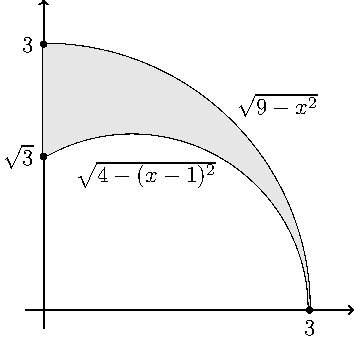
\includegraphics[width=6cm]{./img/CurveTriangle.pdf}
	\end{minipage}
	\hspace{1cm}
	\begin{minipage}{.4\textwidth}
		\centering
		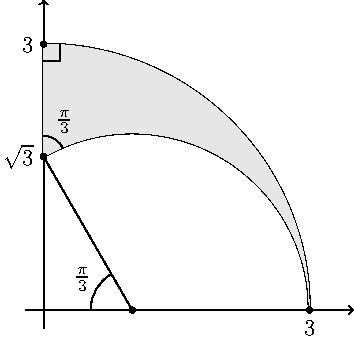
\includegraphics[width=6cm]{./img/CurveAngles.pdf}
	\end{minipage}
	\vspace{.3cm}

	\begin{minipage}{.4\textwidth}
		\centering
		Переход к повторному интегралу
	\end{minipage}
	\hspace{1cm}
	\begin{minipage}{.4\textwidth}
		\centering
		Углы криволинейного треугольника
	\end{minipage}
	
	\caption[format=empty]{}
\end{figure}

